%! Author = Ryan Coslove (rmc326), Shane Ngai (sn718), and Bryan Sun (bs893)
%! Due Date = 12/7/2021

\documentclass{article}

\setlength{\headsep}{0.75 in}
\setlength{\parindent}{0 in}
\setlength{\parskip}{0.1 in}

%=====================================================
% Add PACKAGES Here (You typically would not need to):
%=====================================================

\usepackage{xcolor}
\usepackage[margin=1in]{geometry}
\usepackage{amsmath,amsthm,amssymb,amsfonts}
\usepackage{fancyhdr}
\usepackage{enumitem}
\usepackage{algorithm}
\usepackage{algpseudocode}
\usepackage{graphicx}
\usepackage{xspace}
\usepackage{subcaption}
\usepackage{mathtools}

%=====================================================
% Ignore This Part (But Do NOT Delete It:)
%=====================================================

\theoremstyle{definition}
\newtheorem{problem}{Problem}
\def\fline{\rule{0.75\linewidth}{0.5pt}}
\newcommand{\finishline}{\begin{center}\fline\end{center}}
\newtheorem*{solution*}{Solution}
\newenvironment{solution}{\begin{solution*}}{{\finishline} \end{solution*}}
\newcommand{\thisdate}{December 7, 2021}
\newcommand{\thissemester}{\textbf{Rutgers: Fall 2021}}
\newcommand{\thiscourse}{CS 440: Intro to AI} 
\newcommand{\thishomework}{Number} 
\newcommand{\thisname}{Name} 

\headheight 40pt              
\headsep 10pt
\pagestyle{fancy}

\newcommand{\thisheading}{
   \noindent
   \begin{center}
   \framebox{
      \vbox{\vspace{2mm}
    \hbox to 6.28in { \textbf{\thiscourse \hfill \thissemester} }
       \vspace{4mm}
       \hbox to 6.28in { {\Large \hfill Homework \#\thishomework \hfill} }
       \vspace{2mm}
         \hbox to 6.28in { { \hfill \thisdate  \hfill} }
       \vspace{2mm}
       \hbox to 6.28in {{Names: \thisname \hfill}}
      \vspace{2mm}}
      }
   \end{center}
   \bigskip
}

%=====================================================
% Some useful MACROS (you can define your own in the same exact way also)
%=====================================================


\newcommand{\ceil}[1]{{\left\lceil{#1}\right\rceil}}
\newcommand{\floor}[1]{{\left\lfloor{#1}\right\rfloor}}
\newcommand{\prob}[1]{\Pr\paren{#1}}
\newcommand{\expect}[1]{\Exp\bracket{#1}}
\newcommand{\var}[1]{\textnormal{Var}\bracket{#1}}
\newcommand{\set}[1]{\ensuremath{\left\{ #1 \right\}}}
\newcommand{\poly}{\mbox{\rm poly}}


%=====================================================
% Fill Out This Part With Your Own Information:
%=====================================================
\renewcommand{\thishomework}{3} %Homework number
\renewcommand{\thisname}{Ryan Coslove (rmc326), Shane Ngai (sn718),  Bryan Sun (bs893)} % Enter your name here



\begin{document}

\thisheading
\vspace{-0.75cm}


\begin{problem} %problem 1
	Consider the two-player game described in Figure 1.
	\begin{enumerate}
	\item Draw the complete game tree, using the following conventions:
	\item Write each state as $(s_A, s_B)$ where $s_A$ and $s_B$ denote the token locations.
	\item Put each terminal state in a square box and write its game value in a circle.
	\item Put loop states in double square boxes. Since it's not clear how to assign values to loop states. annotate each with a "?" in a circle.
	\item Now mark each node with its backed-up minimax value (also in a circle). Explain how you handled the "?" values and why.
	\end{enumerate}
	
\end{problem}

\begin{solution}
	\item  

	\begin{figure}[h!]
			\centering
			\IfFileExists{HW3 1.jpg}{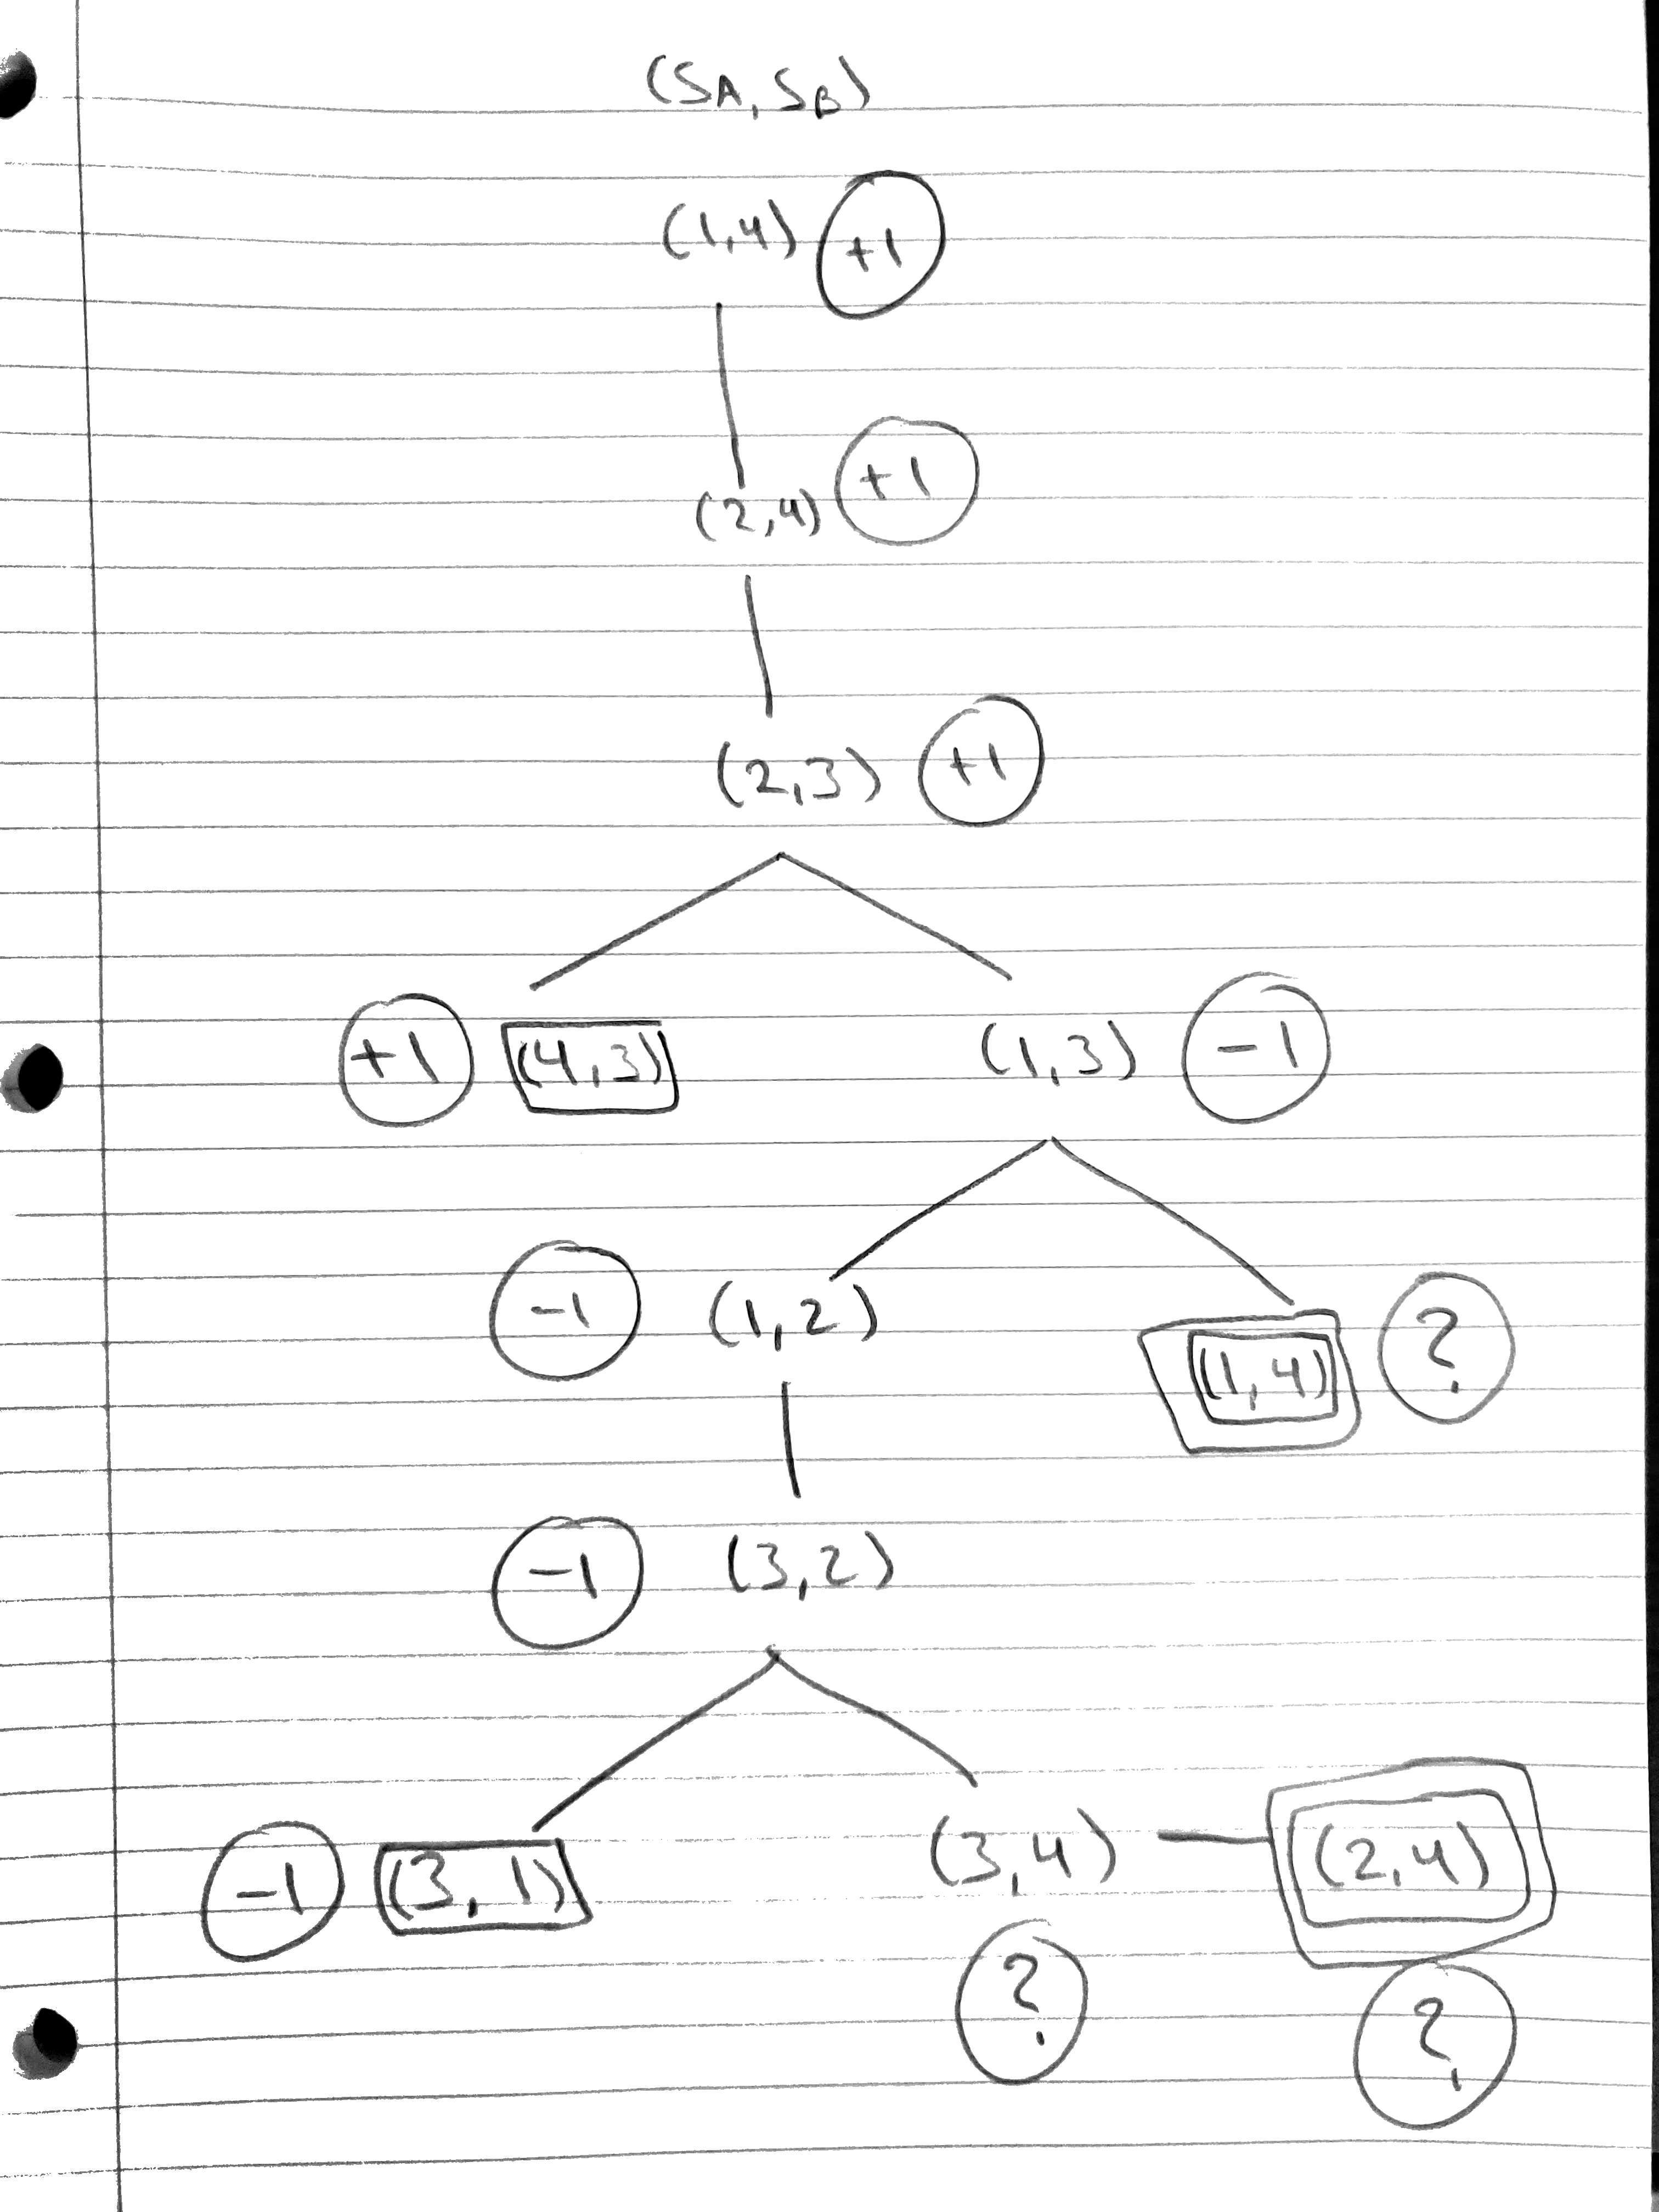
\includegraphics[width=0.6\textwidth]{HW3 1.jpg}}
		 
		\end{figure}
		
	\item The ? values are handled by assuming that the agent has a choice between winning the game and entering a ? state will choose to win. That is min(-1, ?) = -1 and max(+1, ?) = +1. If all successors are ? then the backed up value is ?.

\end{solution}

\begin{problem} %problem 2
	\item Consider the following Bayesian network, where variables A through E are all Boolean valued. Note: there is a typo in the image, it should be P (A = true) = 0.2 instead of P (D = true) = 0.2.
    \item a) What is the probability that all five of these Boolean variables are simultaneously true?
    [Hint: You have to compute the joint probability distribution. The structure of the Bayesian network suggests how the joint probability distribution is decomposed to the conditional probabilities available.]
    \item b) What is the probability that all five of these Boolean variables are simultaneously false?
    [Hint: Answer similarly to above.]
    \item c) What is the probability that A is false given that the four other variables are all known to be true?

\end{problem}

\begin{solution}
	\item 2a)
	\item $P(A,B,C,D,E) = P(A) * P(B) * P(C) * P(D | A,B) * P(E | B,C)$.
	\item $P(A=T,B=T,C=T,D=T,E=T) = P(A=T)*P(B=T)*P(C=T)*P(D=T)*P(E=T) $
	\item $P(A=T,B=T,C=T,D=T,E=T) = 0.2 * 0.5 * 0.8 * 0.1 * 0.3 $
	\item $P(A=T,B=T,C=T,D=T,E=T) = 0.0024$

	\item 2b)
	\item $P(A=F,B=F,C=F,D=F,E=F) = P(A=F)*P(B=F)*P(C=F)*P(D=F)*P(E=F)$
    	\item $P(A=F,B=F,C=F,D=F,E=F) = 0.8 * 0.5 * 0.2 * 0.1 * 0.8 $
        \item $P(A=F,B=F,C=F,D=F,E=F) = 0.0064$

	\item 2c)
	\item $P(\neg A| B,C,D,E)$ 
        \item $\alpha * P(\neg A,B,C,D,E)$
        \item $\alpha =  \frac{1}{P(A,B,C,D,E)+P(\neg A,B,C,D,E)}$
        \item $\alpha = \frac{1}{(0.2 * 0.5 * 0.8 * 0.1 * 0.3)+(0.8 * 0.5 * 0.8 * 0.6 * 0.3)}$
        \item $\alpha = \frac{1}{0.0024+0.0576}$
        \item $\alpha = \frac{50}{3}$
        \item $P(\neg A| B,C,D,E) = \alpha * P(\neg A,B,C,D,E)$
        \item $P(\neg A| B,C,D,E) = \frac{50}{3} * 0.0576$
        \item $P(\neg A| B,C,D,E) = 0.96$

\end{solution}

\begin{problem} %problem 3
	\item a) Calculate $P(Burglary|JohnsCalls = true, MaryCalls = true)$ and show in detail the calculations that take place. Use your book to confirm that your answer is correct.
    \item b) Suppose a Bayesian network has the from of a chain: a sequence of Boolean variables $X_1, . . . X_n$ where $Parents(X_i) = {X_{i-1}}$ for $i = 2, . . . , n$. What is the complexity of computing $P(X_1|X_n = true)$ using enumeration? What is the complexity with variable elimination?

\end{problem}

\begin{solution}
	\item 3a) 
	\begin{align*}
        P(B|J,M) = \frac{P(B,J,M)}{P(J,M)} \\ 
        & = \alpha * P(B) \sum_{E} P(E) \sum_{A} P(A|B,E)*P(J|A)*P(M|A) \ Here, \ (\alpha = \frac{1}{P(J,M)})\\
        & = \alpha * P(B) \sum_{A} P(E) * ((0.9 * 0.7 * \left( \begin{array}{cc} 0.95 & 0.29 \\
0.94 & 0.001 \end{array} \right) + 0.5 * 0.01 * \left( \begin{array}{cc} 1-0.95 & 1-0.29 \\
1-0.94 & 1-0.001 \end{array} \right))\\
        & = \alpha * P(B) \sum_{A} P(E) * ((0.9 * 0.7 * \left( \begin{array}{cc} 0.95 & 0.29 \\
0.94 & 0.001 \end{array} \right) + 0.5 * 0.01 * \left( \begin{array}{cc} 0.05 & 0.71 \\
0.06 & 0.999 \end{array} \right))\\
        & = \alpha * P(B) \sum_{A} P(E) * \left( \begin{array}{cc} 0.598525 & 0.183055 \\
0.59223 & 0.011295 \end{array} \right)\\
        & = \alpha * P(B) * (0.002 * \left( \begin{array}{c} 0.598525 \\ 0.183055 \end{array} \right) + 0.998 * \left( \begin{array}{c} 0.59223 \\ 0.0011295 \end{array} \right)\\
        & = \alpha * \left( \begin{array}{c} 0.001 \\ 0.999 \end{array} \right) * \left( \begin{array}{c} 0.59224259 \\ 0.001493351 \end{array} \right)\\
        & = \alpha * \left( \begin{array}{c} 0.00059224259 \\ 0.0014918576 \end{array} \right)\\
        & ( We \ can \ calculate \ \alpha  \ the \ using \ the \ same \ method. \ \alpha = \frac{1}{0.0020853609})\\ 
        & = \frac{1}{0.0020853609} * \left( \begin{array}{c} 0.00059224259 \\ 0.0014918576 \end{array} \right) \\
        & = <0.284, 0.716>
    \end{align*}  

	\item 3b) 
	\item First, we evaluate two binary trees for each value of $X_{1}$ and each of them have the depth $n - 2$. Therefore, the total work for enumeration will be $O(2_{n})$.
	\item Next, variable elimination. In variable elimination, the factors will never grow more than two variables. For example,
    	\item \begin{align*}
    	P(X_{1} | X_{n} = True) 
    	& = \alpha * P(X)  \ ...\sum_{x_{n-2}} P(x_{n-2} | x_{n-3}) \sum_{x_{n-1}} P(x_{n-1} | x_{n-2}) P(X_{n} = True | x_{n-1})\\
    	& = \alpha * P(X) \ ... \sum_{x_{n-2}} P(x_{n-2} | x_{n-3}) \sum_{x_{n-1}} f X_{n-1}(x_{n-1}, x_{n-2}) f X_{n}(x_{n-1})\\
	& = \alpha * P(X) \ ... \sum_{x_{n-2}}P(x_{n-2} | x_{n-3}) f \frac{x_{n-2}}{X_{n-1}* X_{n}}
    \end{align*}
	\item  As we see here, this is isomorphic to the problem $n-1$ variables and not $n$. Therefore the work done will be a constant independent of $n$ and the total work is $O(n)$.

\end{solution}

\begin{problem} %problem 4
		\item Suppose you are working for a financial institution and you are asked to implement a fraud detection system. You plan to use the following information:
	\begin{itemize} 
	    \item When the card holder is travelling abroad, fraudulent transactions are more likely since tourists are prime targets for thieves. More precisely, 1\% of transactions are fraudulent when the card holder is travelling, where as only 0.4\% of the transactions are fraudulent when she is not travelling. On average, 5\% of all transactions happen while the card holder is travelling. If a transaction is fraudulent, then the likelihood of a foreign purchase increases, unless the card holder happens to be travelling. More precisely, when the card holder is not travelling, 10\% of the fraudulent transactions are foreign purchases where as only 1\% of the legitimate transactions are foreign purchases. On the other hand, when the card holder is travelling, then 90\% of the transactions are foreign purchases regardless of the legitimacy of the transactions.
	    \item Purchases made over the internet are more likely to be fraudulent. This is especially true for card holders who don’t own any computer. Currently, 75\% of the population owns a computer or smart phone and for those card holders, 1\% of their legitimate transactions are done over the internet, however this percentage increases to 2\% for fraudulent transactions. For those who don’t own any computer or smart phone, a mere 0.1\% of their legitimate transactions is done over the internet, but that number increases to 1.1\% for fraudulent transactions. Unfortunately, the credit card company doesn’t know whether a card holder owns a computer or smart phone, however it can usually guess by verifying whether any of the recent transactions involve the purchase of computer related accessories. In any given week, 10\% of those who own a computer or smart phone purchase (with their credit card) at least one computer related item as opposed to just 0.1\% of those who don’t own any computer or smart phone.
\end{itemize} 

    \item a) Construct a Bayes Network to identify fraudulent transactions.
What to hand in: Show the graph defining the network and the Conditional Probability Tables associated with each node in the graph. This network should encode the information stated above. Your network should contain exactly six nodes, corresponding to the following binary random variables: 
    \item OC : card holder owns a computer or smart phone.
    \item Fraud : current transaction is fraudulent.
    \item Trav : card holder is currently travelling.
    \item FP : current transaction is a foreign purchase.
    \item IP : current purchase is an internet purchase.
    \item CRP : a computer related purchase was made in the past week.
    \item The arcs defining your Network should accurately capture the probabilistic dependencies between these variables.
    \item b) What is the prior probability (i.e., before we search for previous computer related purchases and before we verify whether it is a foreign and/or an internet purchase) that the current transaction is a fraud? What is the probability that the current transaction is a fraud once we have verified that it is a foreign transaction, but not an internet purchase and that the card holder purchased computer related accessories in the past week? What to hand in: Indicate the two queries (i.e., $Pr(variables|evidence))$ you used to compute those two probabilities. Show each step of the calculation
\end{problem}

\begin{solution}
	\item  4a)

	\begin{figure}[h!]
			\centering
			\IfFileExists{HW3 4.png}{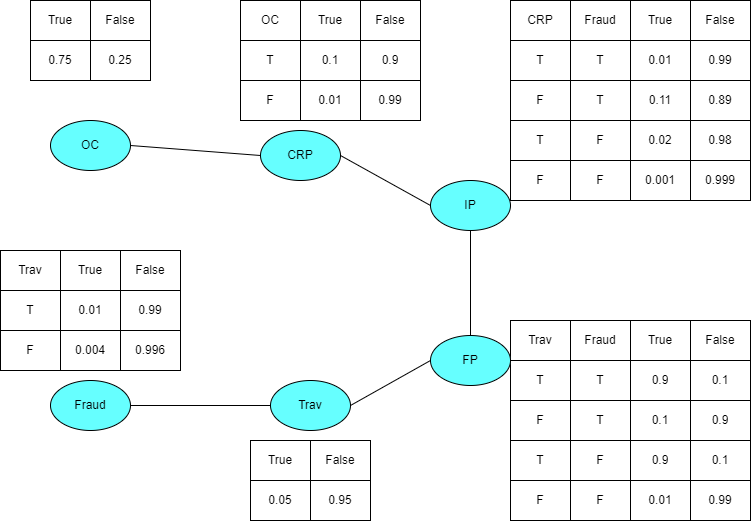
\includegraphics[width=0.9\textwidth]{HW3 4.png}}
		 
		\end{figure}

	\item 4b)
	\item 
	\begin{align*}
	P(Fraud)
		& = P(Fraud=T|Trav=T) * P(Trav =T) + P(Fraud=T|Trav=F) * P(Trav = F) \\
		& = 0.01 * 0.05 + 0.004 * 0.95 \\
		& =0.004275 \\
	\end{align*}

	\begin{align*}
	P(Fraud|FP)
				&=P(Fraud |Trav) P(FP|Trav,Fraud) P(Trav) +\\
				&+ P(Fraud|\neg Trav)P(FP|\neg Trav, Fraud)P(\neg Trav)\\
				&=0.01 *0.90 *0.05 + 0.004* 0.10* 0.95\\
				&=0.00045 + 0.00038\\
				&=0.00083\\
	\end{align*}

	\begin{align*}
	P(Fraud|\neg IP,CRP, OC)
		&= P(\neg IP|CRP,Fraud) P(CRP) + P(\neg IP|\neg CRP,Fraud)P(\neg CRP)\\
		&= P(\neg IP|CRP,Fraud) * (P(CRP|OC)*P(OC) + P(CRP|\neg OC)*P(\neg OC)) \\
		&+ P(\neg IP|\neg CRP,Fraud)* (P(\neg CRP|OC)*P(OC) + P(\neg CRP|\neg OC)*P(\neg OC))\\
		&=0.99*(0.1*0.75+0.01*0.25)+0.89*(0.9*0.75+0.99*0.25)\\
		&=0.99*0.02125+0.89*0.41625\\
		&=0.379\\
	\end{align*}
\item $P = 0.379 * 0.00083 = 0.00031457$


\end{solution}


\end{document}